
In this section I justify the design choices made for the implementation of the given system description. The goal was to build an efficient and stable system while still keeping it simple to analyze. 

\subsection{Overall architecture}
The main components of the system are the net-thread (\texttt{NetThread.java}), the requests  (\texttt{Request.java}) and the worker threads (\texttt{WorkerThread.java}), which will be explained in more detail in the following subsections. \\

\begin{figure}[!h]
    \centering
	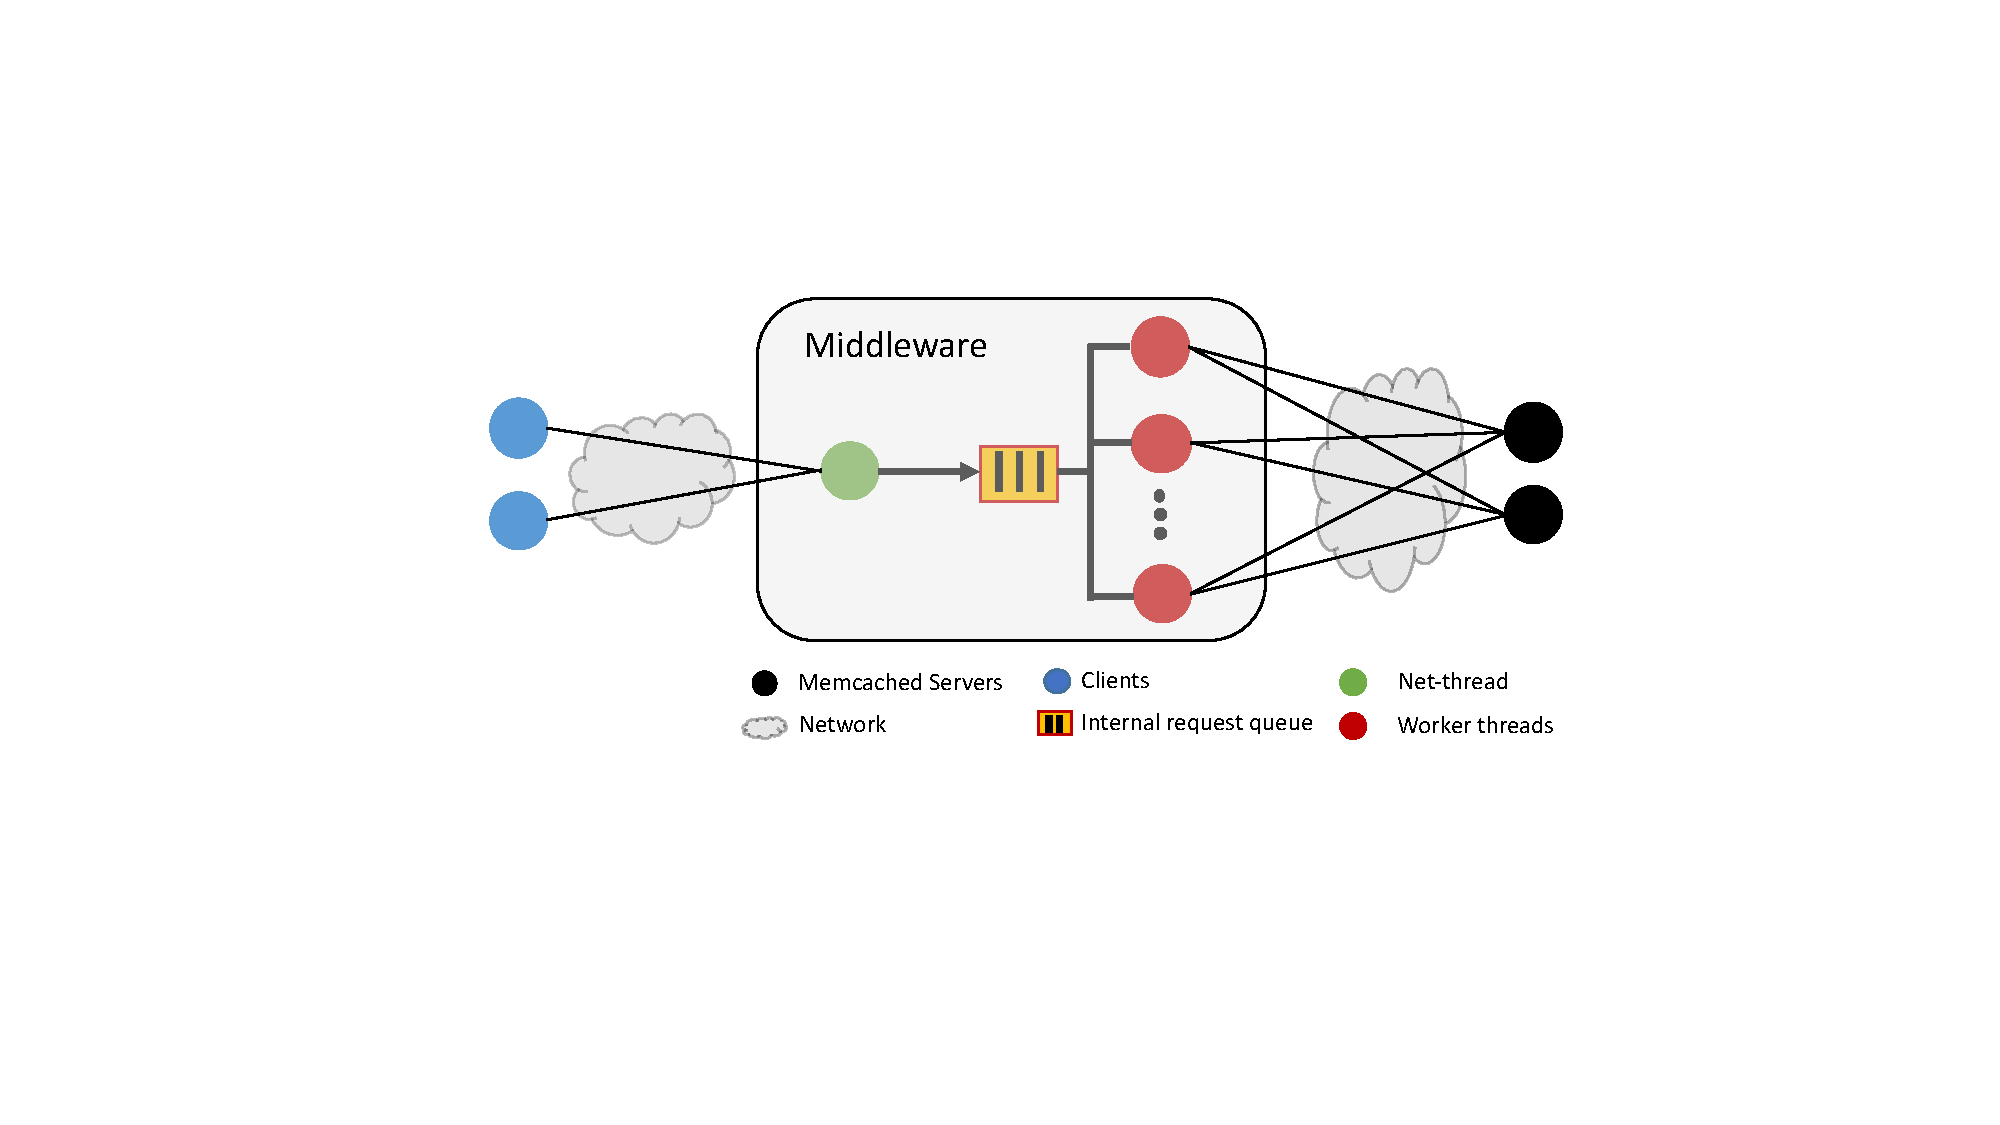
\includegraphics[scale=0.7]{figures/0_SystemOverview/overview_figure.pdf}
	\caption{Interaction between components of the system.}
	\label{overview}
\end{figure}

Figure \ref{overview} gives a simplified overview of the system. First, a client sends a request over a TCP connection to the net-thread. The net-thread reads the message into a buffer, encapsulates it into a \textit{Request} object and puts it into an internal request queue. An available worker thread takes out a request from the queue (if there is one) and processes it depending on its type. The request is sent over a TCP connection to one or multiple servers, after which their response is read into a buffer, then processed and sent back to the client. \\

\texttt{RunMW.java} is the entry point of the system. It parses the command line arguments, such as the addresses of the memcached servers, the address of the net-thread and the number of worker threads in the system. It starts the Middleware by creating an instance of the \textit{Middleware} class, which then starts the worker threads and the net-thread. 

\subsection{Net-Thread}
The \texttt{NetThread} class extends the \textit{Thread}\footnote{\url{https://docs.oracle.com/javase/8/docs/api/java/lang/Thread.html}} class. 
The net-thread basically does two things: It establishes client connections and puts received requests into a queue. \\

% client connections
A \textit{Selector}\footnote{\url{https://docs.oracle.com/javase/8/docs/api/java/nio/channels/Selector.html}} is used to handle multiple connections with a single thread. A selector can monitor multiple connections for certain I/O events and notify the net-thread when they occur. At first, the net-thread creates a server socket channel which it binds to its address. This channel's sole purpose is to accept new connections from clients. It is registered with the selector for "accept events", i.e. the selector monitors incoming connections on the server socket channel. When this event happens, the net-thread gets notified by the selector and creates a new socket channel for the connection to the client. New socket channels are registered with the selector for "read events", i.e. the selector monitors when data from the clients is ready to be read from. Again, when this event occurs, the net-thread gets notified and reads the data. Note that the net-thread has to call the blocking \textit{select()} method on the selector to be notified for those events.\\
% why Selector, advantages, consequences, non-blocking I/O
This design allows the net-thread to monitor multiple channels for I/O events at the same time. It also enables non-blocking I/O between the clients and the net-thread without having the net-thread to constantly poll the medium and wasting CPU resources. \\

% buffer
We want to minimize the number of times we allocate \textit{ByteBuffer}\footnote{\url{https://docs.oracle.com/javase/8/docs/api/java/nio/ByteBuffer.html}} objects and reuse them as often as possible to minimize both data copy operations and memory allocation on the heap. The net-thread only needs to allocate one buffer per client connection because we have a closed system, i.e. clients wait for a response before sending the next request. Therefore, before sending a response to the client, we just clear the buffer associated with this client connection such that it can be reused again for a new request from this client. Since we have a fixed number of clients, the number of buffer allocations by the net-thread is also fixed and does not grow with the number of request. \\
We associate a buffer with each client connection using the \textit{SelectionKey}\footnote{\url{https://docs.oracle.com/javase/8/docs/api/java/nio/channels/SelectionKey.html}} object. A selection key is created whenever we register a channel with a selector. Most importantly, it contains the channel for which the key was created and an attachment where we can store any object. We use this attachment to associate a buffer with each client connection. \\

% request enqueueing
Whenever a full request has been read into a byte buffer by the net-thread, it encapsulates it in a \textit{Request} object and puts it into the internal request queue. More details about the \textit{Request} class and the queue will be given in the next subsection. 

\subsection{Requests}
% LinkedBlockingQueue (why, advantages -> unbounded?, thread safe, take out is blocking, add non-blocking)
There are several reasons why we have chosen a \textit{LinkedBlockingQueue}\footnote{\url{https://docs.oracle.com/javase/8/docs/api/java/util/concurrent/LinkedBlockingQueue.html}} to enqueue and dequeue requests. First of all, we use a blocking queue because the \textit{take()} operation should block until an element becomes available, which is more efficient (in terms of CPU usage) than constantly polling the queue and checking if an element is in there. \\
We use the linked implementation (in contrast to the array implementation) because of the following reasons: We have constant time for the take() and put() operation because doubly-linked nodes are used as an internal data structure. There is a separate lock for the head and the tail, which may result in better throughput because we can add and remove elements simultaneously. The default capacity is \mintinline{java}{Integer.MAX_VALUE}, which can be considered unbounded. That's good because we don't know how many requests may be in the queue and also we don't have to allocate space for requests a priori as for the \textit{ArrayBlockingQueue}. \\
However, there is a disadvantage in choosing the linked blocking queue, namely that the performance may be more variable than with an array blocking queue because of the dynamic allocation of nodes during usage and the more complicated data structure with doubly-linked nodes. \\

% explain fields
Requests from clients are encapsulated in \textit{Request} objects. The \textit{Request} class contains the following fields: 
\begin{itemize}
    \item \textbf{buffer}: The byte buffer into which the request from the client was written into.
    \item \textbf{key}: A selection key which contains the channel over which the request was sent to the net-thread. This channel is used by the worker threads to be able to send the response back to the correct client. 
    \item \textbf{type}: The type of the request which is either a Set, a Get (includes Multiget) or an Invalid request. 
    \item \textbf{instrumentation fields}: See subsection \ref{sub:instr}.
\end{itemize}
% explain parseMethod
The constructor of the \textit{Request} class calls a method \textit{parseRequest()}, which first checks if there is an end of line string \texttt{\textbackslash r\textbackslash n} at the last two written bytes of the byte buffer. If there is none, the request is considered Invalid. Then the type of the request is determined based on the first three chars of the request which should be either 'get' or 'set'. Note that the distinction between Multiget and Get requests is not done at this point in order to avoid code duplication and keeping the code simple. 

\subsection{Worker Threads}
% role of worker threads, what do they do
The \texttt{WorkerThread} class extends the \textit{Thread}\footnote{\url{https://docs.oracle.com/javase/8/docs/api/java/lang/Thread.html}} class. 
The role of the worker threads is basically to establish connections to the memcached servers and to process the requests that the net-thread added to the internal request queue. \\

% First: memcached server connections (blocking)
The first thing a worker thread does is to establish a permanent connection to each memcached server. The addresses of those servers are passed as an argument to the middleware at start-up. A worker thread opens a socket channel for each server and connects it to the server. The socket channels are stored in an array list, in order to be able to access them later on. The channels are configured to be blocking to keep the code simple and to not waste CPU resources while polling until a whole response has been read from a server. However, it also has disadvantages like failure during blocking calls leading to unresponsiveness and scalability issues if we have a lot of open connections, which in our case we don't have because we can have at maximum three servers. \\

% write about buffers (efficient allocation and reusability of responseBuffer)
For the buffer allocations, once again, we want to use as few allocations as possible and reuse them. This is achieved by having each worker thread allocating one buffer and referencing it with a field. This buffer is used to write the response from the servers into. If a request is done being processed, the buffer can be cleared in order to be reused again. Note that because of the sharded mode we actually allocate another buffer to make the reassembly of the responses easier, which will be explained later in more detail. But still the number of buffers doesn't grow with the number of requests and stays proportional to the number of worker threads.\\

The main loop of the worker thread consists of taking out a request from the queue (this is a blocking operation), processing it depending on its type and when finished taking out another one and so forth. \\
If the type of the request is \mintinline{java}{SET} then it will call \textit{handleSetRequest()}, if it is \mintinline{java}{GET} then it will call \textit{handleGetReuquest()} and if it is \mintinline{java}{INVALID}, it will send the error message "\mintinline{java}{ERROR}\texttt{\textbackslash r\textbackslash n}" to the client having sent the request.

% two subsubsections: different kind of requests (set and get request): explain each execution path in detail
\subsubsection{Handle a Set Request}
For a Set request, the worker thread sends it to each server and then waits for a response of all of them. If one or multiple servers respond with an error message, one of them is forwarded to the client. If no error occurred, one of the success messages is forwarded to the client. \\
This is implemented as follows: The buffer contained in the \textit{Request} object is sent sequentially to each server by iterating over the socket channels. After that, we go over the socket channels again and for each socket channel we write the response into our buffer and check the content in order to find out if the Set request was successfully executed on the server. If it was not, the error message is added to an array list. Note that we always read from a channel until we get an end of line string, which denotes that a full response has been read. And also note that the buffer is cleared before writing into it, such that we can reuse it and not have to allocate a new one for each response. After having processed all responses, if there occurred an error, we just forward the first error message to the client and otherwise the last success message is forwarded to the client because it is still contained in the buffer. 

\subsubsection{Handle a Get Request}
For the \textbf{non-sharded mode}, we just forward the Get request (includes Multiget requests) to one server, which is chosen based on a round-robin scheme, and the response from the server is forwarded to the client. We don't have to inspect the response because independently of success or error, it can always be forwarded to the client. \\
The round-robin scheme works by having a private field \textit{'lastServerIndex'} in each worker thread,  which identifies the last server used by this worker thread for a Get request. Whenever a worker thread sends a (non-sharded) Get request, it executes the following code to retrieve the socket channel it uses to write the request to. Note that \textit{'socketChannels'} is an array list containing all established socket channels to the servers.   
\begin{minted}[frame=single]{java} 
    lastServerIndex = (lastServerIndex + 1) % socketChannels.size();
    SocketChannel socketChannel = socketChannels.get(lastServerIndex);
\end{minted}
 The empirical evaluation of the load balancing and the justification of this design choice is given in subsection \ref{sub:lb}. \\
  
For the \textbf{sharded mode}, a Multiget request has to be evenly split into a set of smaller Multiget requests, one for each server. Note that if there are fewer keys in the request than servers, we need to load balance them such that whenever this case occurs, not always the same servers are hit. To simplify the explanation, we ignore this case for the moment. \\
First we extract the keys from the request and put them into the '\textit{keys'} array. There can be between 1 and 10 keys. Each server is identified with an index which corresponds to the position of its socket channel in the \textit{'socketChannels'} array. We then need to figure out the number of keys each server should handle such that they are evenly distributed and sum up to the total number of keys in the \textit{'keys'} array. We do this based on the index which identifies a server: 
\begin{minted}[frame=single]{java}
    public static int getKeyCount(int index, int numKeys, int serverCount) {
        int keyCount = 0;
        for (int i = index; i < numKeys; i += serverCount) {
            keyCount++;
        }
        return keyCount;
    }
\end{minted}
\textit{getKeyCount()} is a method that returns the number of keys for which a server with a specific index is responsible for. \textit{'numKeys'} is the total number of keys in the request and \textit{'serverCount'} is the total number of servers. It works by counting how many times we can add the 'serverCount' to the index until we exceed the 'numKey'. For example if we have 3 servers and 7 keys, index 0 gets 3 keys, index 1 gets 2 keys and index 2 gets 2 keys which sums up to 7 keys and is evenly distributed. \\
For each server we do the following: Construct the Get request based on its \textit{'getKeyCount()'}. The keys are retrieved from the \textit{'keys'} array in-order, i.e. the server with index 0 retrieves the first n elements, then the server with index 1 retrieves the next m elements and so on. \\
After all Get requests have been sent, we retrieve the responses from the servers in the same order as we have sent the requests, which simplifies the reassembly of the responses. The responses are reassembled into one response in a separate buffer for simplicity. In case of an error message, an error flag is raised and in the end '\mintinline{java}{ERROR}\texttt{\textbackslash r\textbackslash n}' is sent to the client instead of the reassembled response. \\
What is left to explain is how we handle the case with fewer keys than servers. Since we don't want to always hit the first n servers in the \textit{'socketChannels'} array, where n is the number of keys, we apply the same round-robin scheme as in the non-sharded mode. But now we need to keep track of which servers we queried and in which order we did it, in order to be able to reassemble the responses in the correct order. For this we use an array called \textit{'usedServers'}. The value of \textit{'usedServers'} at position i tells if we did send a request to a server at iteration i, and if yes to which we did send one. 

\subsection{Load Balancing} \label{sub:lb}
% design choice
To denote the last server used in the round-robin scheme, we have chosen to use a private field \textit{'lastServerIndex'} in each worker thread instead of a global variable because it avoids having to synchronize access on it. Having all worker threads access the same variable for every Get request concurrently would lead to blocking behavior, which degrades the performance. 

% empirical evaluation -> show plot
We did an empirical evaluation to show that on average all memcached servers are subject to the same load. The experiment was run on the cluster with 1 client, 4 worker threads and 3 memcached servers with Get requests only. Each worker thread printed how many times it hit each of the servers:
\begin{lstlisting}[basicstyle=\tiny]                
[Thread-2] ch.ethz.asl.WorkerThread: [0=16208, 1=16208, 2=16208] 
[Thread-4] ch.ethz.asl.WorkerThread: [0=15208, 1=15209, 2=15208] 
[Thread-5] ch.ethz.asl.WorkerThread: [0=15753, 1=15754, 2=15753] 
[Thread-3] ch.ethz.asl.WorkerThread: [0=16307, 1=16308, 2=16308] 
\end{lstlisting}
Server 0 was hit 63'476 times, server 1 was hit 63'479 times and server 2 was hit 63'477 times which shows that the load is distributed equally among the servers.

\subsection{Instrumentation} \label{sub:instr}
The following timestamps are collected during the lifetime of a request:
\begin{itemize}
    \item \textbf{timeFirstByte}: Time at which the first byte of the request is read by the net-thread.
    \item \textbf{timeEnqueued}: Time at which the request is enqueued into the internal request queue by the net-thread. 
    \item \textbf{timeDequeued}: Time at which a worker thread dequeues the request from the internal request queue.
    \item \textbf{timeMemcachedSent}: Time immediately before the worker thread sends the (first) request to a memcached server. 
    \item \textbf{timeMemcachedReceived}: Time immediately after the (last) response of a memcached server was read by the worker thread. 
    \item \textbf{timeCompleted}: Time at which the worker thread sends the response back to the client. 
\end{itemize}
All those timestamps, the queue length after the request is dequeued and the request type is stored in the \textit{Request} object itself. After the request is completed, the worker calls the method \textit{writeLogLine()} on it, which writes the instrumentation data to a csv-file. Note that we use \textit{Log4j} for logging, which is configured to not immediately flush on each \textit{log()} invocation, but buffers the logs until its capacity of 8'192 bytes is reached. We compared experiments with and without logging in order to check that logging does not affect the performance of the middleware. 

Aggregation of log-files is outsourced to python scripts which run after the experiments are finished. A more detailed explanation of the postprocessing can be found in the \textit{README} files of the repository.